% =====================================================================
%  Project report -- IEEE conference format (IEEEtran).
%  Overleaf: New Project -> Upload Project -> select report_overleaf.zip
%  Local:    pdflatex main && pdflatex main
% =====================================================================
\documentclass[conference]{IEEEtran}
\IEEEoverridecommandlockouts

\usepackage{cite}
\usepackage{amsmath,amssymb,amsfonts}
\usepackage{graphicx}
\usepackage{booktabs}
\usepackage{multirow}
\usepackage{xcolor}
\usepackage{url}
\usepackage[hidelinks]{hyperref}

\newcommand{\G}[1]{\textsf{#1}}

\begin{document}

\title{Learning Battery Dispatch Across Heterogeneous Microgrids:\\
A Reinforcement Learning Study Against LP and MPC Baselines}

\author{
\IEEEauthorblockN{Shreyansh Mishra, Aryan Sawant, Ankit Yadav, Chirag Bhut, Mihika Chawda, Nitesh Funde}
\IEEEauthorblockA{\textit{Department of Artificial Intelligence}\\
\textit{Sardar Vallabhbhai National Institute of Technology (SVNIT)}\\
Surat, India}
}

\maketitle

\begin{abstract}
Reinforcement learning (RL) for battery energy management is usually evaluated
on a single site, with a single tariff, a few days of data and no closed-loop
baseline. That makes it hard to know whether a result says anything about RL
or only about one configuration. We first reproduce the usual setting, a 13.5\,kWh
residential battery under a time-of-use tariff, and then extend it to six
microgrid archetypes driven by a full year of real 2018 data: hot- and
cold-climate homes, a commercial office with a demand charge, a capacity-limited
rural feeder, an electric-vehicle community on wholesale real-time prices, and
an industrial warehouse. To make multi-site training practical on a laptop
GPU, we implement the microgrid as a batched PyTorch environment
(${\sim}2.3$M environment steps/s) together with custom Soft Actor-Critic (SAC)
and Proximal Policy Optimisation (PPO) agents. We compare them with a
perfect-foresight linear program (LP), an hourly model-predictive controller
(MPC) and two heuristics on held-out test days. A per-grid SAC captures 67--97\,\% of the
LP's savings on five of the six grids, and one generalist SAC policy loses only
2--6 points on those five. Policies trained on five grids do not transfer
zero-shot to the sixth. Under 30\,\% correlated forecast error, the open-loop LP
collapses on real-time prices ($-191$\,\%), MPC is best on the residential and
real-time-price grids, and a domain-randomised SAC is best where demand
charges and grid caps punish forecast errors. The best controller therefore
depends on the site, a conclusion that a single-site study cannot reach.
\end{abstract}

\begin{IEEEkeywords}
battery energy storage, microgrid, energy management, deep reinforcement
learning, soft actor-critic, model predictive control, forecast uncertainty,
generalisation
\end{IEEEkeywords}

% ---------------------------------------------------------------------
\section{Introduction}

Behind-the-meter batteries earn money in different ways depending on where they
are installed. A home on a time-of-use (TOU) tariff buys cheap night energy and
avoids the evening peak. An office pays a demand charge on its largest kW of
the day. A rural community on a weak feeder must avoid shedding load. An
electric-vehicle (EV) community on real-time prices chases a price curve that
changes every day. The controller has to make an hourly decision under uncertain
load and solar forecasts in every case, but the structure of the problem changes
with the site.

Deep RL is an attractive controller for this setting because it re-decides every
hour from the current state and needs no explicit optimisation model at run
time~\cite{vazquez2019review}. Most RL energy-management studies, however,
evaluate one building with one tariff over a short horizon, and compare against
heuristics or against an LP with perfect foresight but not against a closed-loop
MPC~\cite{parisio2014mpc}. A single configuration cannot show whether a learned
controller generalises, and without MPC there is no fair answer to the question
of whether RL is needed at all.

This project started from that usual setting: SAC~\cite{haarnoja2018sac}, PPO~\cite{schulman2017ppo}
and a domain-randomised SAC trained with Stable-Baselines3~\cite{raffin2021sb3} on a single residential
day. Following feedback that the study should reflect real-world variety, we
extended it to a multi-grid benchmark. Our contributions are:
\begin{itemize}
\item \textbf{Six microgrid archetypes} with real 2018 hourly data: NREL
End-Use Load Profiles~\cite{wilson2022eulp}, PV computed from NREL weather, and
NYISO wholesale prices. Each archetype has its own battery, PV, tariff and grid-connection
limits (Table~\ref{tab:grids}), and every month is split into
training, validation and test days.
\item \textbf{A GPU-batched environment} that reproduces the original Gymnasium
environment exactly (verified by test) while adding separate import and export prices,
demand charges, import caps with value of lost load (VoLL) and export curtailment.
It runs ${\sim}2.3$M steps/s on an RTX~3050 laptop GPU, against
${\sim}80$ steps/s for the original setup.
\item \textbf{Strong baselines}: an LP whose objective equals the environment's
daily cost exactly, the same LP run open loop on forecasts, and a
shrinking-horizon MPC.
\item \textbf{Four experiments}, covering per-grid specialists (E1), one generalist
policy (E2), zero-shot transfer to an unseen grid (E3), and robustness to
correlated forecast error (E4). We also release an interactive dashboard with a
grid selector.
\end{itemize}

% ---------------------------------------------------------------------
\section{Related Work}

\textit{Optimisation-based dispatch.} With known profiles, battery scheduling is
a linear program; under uncertainty, MPC re-solves it on a receding horizon and
is the de-facto industrial baseline for microgrid operation~\cite{parisio2014mpc}.
We use the HiGHS solver~\cite{huangfu2018highs} for both.

\textit{RL for energy management.} Reviews of RL for demand response
document a wide spread of algorithms and settings and a lack of common
benchmarks~\cite{vazquez2019review}. CityLearn~\cite{vazquez2019citylearn}
introduced a multi-building Gym environment, but it targets district-level
coordination rather than heterogeneous single-site tariffs and grid limits.
Off-policy actor-critic methods such as SAC~\cite{haarnoja2018sac} and on-policy
PPO~\cite{schulman2017ppo} with GAE~\cite{schulman2016gae} are the most common choices.

\textit{Generalisation and robustness.} RL policies are known to overfit their
training environments~\cite{cobbe2019quantifying}, and reported results are
sensitive to seeds and implementation details~\cite{henderson2018matters}.
Domain randomisation~\cite{tobin2017domain} trains on perturbed environments to
gain robustness. We apply it to forecast error. GPU-batched simulation, popularised
by Isaac Gym~\cite{makoviychuk2021isaac}, makes multi-configuration training affordable.

% ---------------------------------------------------------------------
\section{System Model}

\subsection{Microgrid and cost}
Each microgrid has an aggregate load $L_t$, a PV output $S_t$, and a battery with
capacity $E^{\max}$, power limit $\bar P$, ramp limit $R$, charge and discharge
efficiencies $\eta_c=\eta_d=0.95$ and a minimum state of charge (SOC) of 10\,\%. The agent chooses battery
power $P^b_t\in[-\bar P,\bar P]$ (positive means charging) once per hour of a
24\,h day. After the ramp, SOC and grid-limit checks, the grid exchange is
\begin{equation}
P^g_t = L_t - S_t + P^b_t - U_t + C_t ,
\end{equation}
where $U_t\ge 0$ is load shed above an import cap $\bar P^{\mathrm{imp}}$ and
$C_t\ge 0$ is PV curtailed above an export cap $\bar P^{\mathrm{exp}}$. The battery energy follows
$E_{t+1}=E_t+\eta_c[P^b_t]^+ - [P^b_t]^-/\eta_d$. The hourly cost is
\begin{align}
c_t ={}& \pi^{\mathrm{imp}}_t [P^g_t]^+ - \pi^{\mathrm{exp}}_t [P^g_t]^-
 + \lambda^{\mathrm{pk}} [P^g_t-\bar P^{\mathrm{pk}}]^+ \nonumber\\
 &+ \kappa^{\mathrm{dc}}\big([P^g_t]^+ - M_{t-1}\big)^+ + \mathrm{VoLL}\,U_t \nonumber\\
 &+ \kappa^{\mathrm{deg}} |E_{t+1}-E_t| ,
\end{align}
with $M_t=\max(M_{t-1},[P^g_t]^+)$ the running peak import. Charging the demand
charge incrementally makes the daily total equal to
$\kappa^{\mathrm{dc}}\max_t [P^g_t]^+$ while keeping the reward dense. A terminal
penalty $\kappa^{T}E^{\max}|\mathrm{SOC}_{24}-0.5|$ stops the agent from draining
the pack for a one-day gain. The reward is $-c_t$, scaled by the grid's
$E^{\max}\bar\pi^{\mathrm{imp}}$ during training only; all reported numbers are in
real dollars.

\subsection{Archetypes and data}
Table~\ref{tab:grids} lists the six archetypes. \G{G1} reproduces the original
single-home configuration exactly. The archetypes were chosen so that each one
rewards a different behaviour: TOU arbitrage (\G{G1}), pure PV
self-consumption under a flat tariff (\G{G2}), peak shaving under a demand
charge (\G{G3}, \G{G6}), avoiding lost load on a 30\,kW feeder (\G{G4}), and
real-time price tracking with no export (\G{G5}).

All data are hourly for calendar year 2018:
\begin{itemize}
\item \textbf{Loads.} Taken from NREL ResStock and ComStock (AMY2018)~\cite{wilson2022eulp}. Residential grids sum individual homes, filtered by annual consumption, and commercial grids scale the county building-type aggregate to the target floor area.
\item \textbf{PV.} Computed from the same NREL county weather files (GHI, DNI, DHI and temperature) with a PVWatts-style model~\cite{dobos2014pvwatts}, so load and generation share the same weather.
\item \textbf{Prices.} \G{G5} uses NYISO NYC day-ahead zonal LBMP~\cite{nyiso} plus a \$0.10/kWh delivery adder.
\item \textbf{EV load.} \G{G5}'s eight EV charging profiles are synthesised from arrival-time and energy distributions, because no matching public 2018 session data exist.
\item \textbf{Split.} Within every month, days 8--14 are test days, days 22--28 are validation days and the rest are training days, so every split covers all seasons. \G{G1} and \G{G2} have three independent home profiles each, which gives 252 test days for them and 84 for the other grids.
\end{itemize}
Fig.~\ref{fig:data} shows typical winter and summer days.

\begin{table*}[t]
\centering
\caption{Microgrid archetypes (all data: calendar year 2018). DC = demand charge.}
\label{tab:grids}
\setlength{\tabcolsep}{4pt}
\resizebox{\textwidth}{!}{%
\begin{tabular}{llrrrll}
\toprule
ID & Archetype (location) & Battery & PV & Mean load & Tariff & Grid limits \\
\midrule
G1 & Residential, hot (Austin) & 13.5 kWh / 5 kW & 6 kWp & 1.2 kW & res.\ TOU, 40\,\% feed-in & soft peak 10 kW \\
G2 & Residential, cold (Minneapolis) & 10 kWh / 5 kW & 5 kWp & 0.9 kW & flat \$0.14, 25\,\% feed-in & -- \\
G3 & Commercial office (Los Angeles) & 200 kWh / 60 kW & 120 kWp & 100.1 kW & commercial TOU & DC \$0.60/kW-day \\
G4 & Rural weak grid, 20 homes (AZ) & 200 kWh / 40 kW & 80 kWp & 17.2 kW & flat \$0.12 & imp./exp.\ $\le$ 30 kW, VoLL \$5/kWh \\
G5 & EV community, 10 homes + 8 EVs (NY) & 60 kWh / 25 kW & 40 kWp & 10.6 kW & NYISO LBMP + \$0.10 & no export \\
G6 & Industrial warehouse (Houston) & 500 kWh / 125 kW & 300 kWp & 157.8 kW & industrial TOU & DC \$1.00/kW-day \\
\bottomrule
\end{tabular}}
\end{table*}

\begin{figure*}[t]
\centering
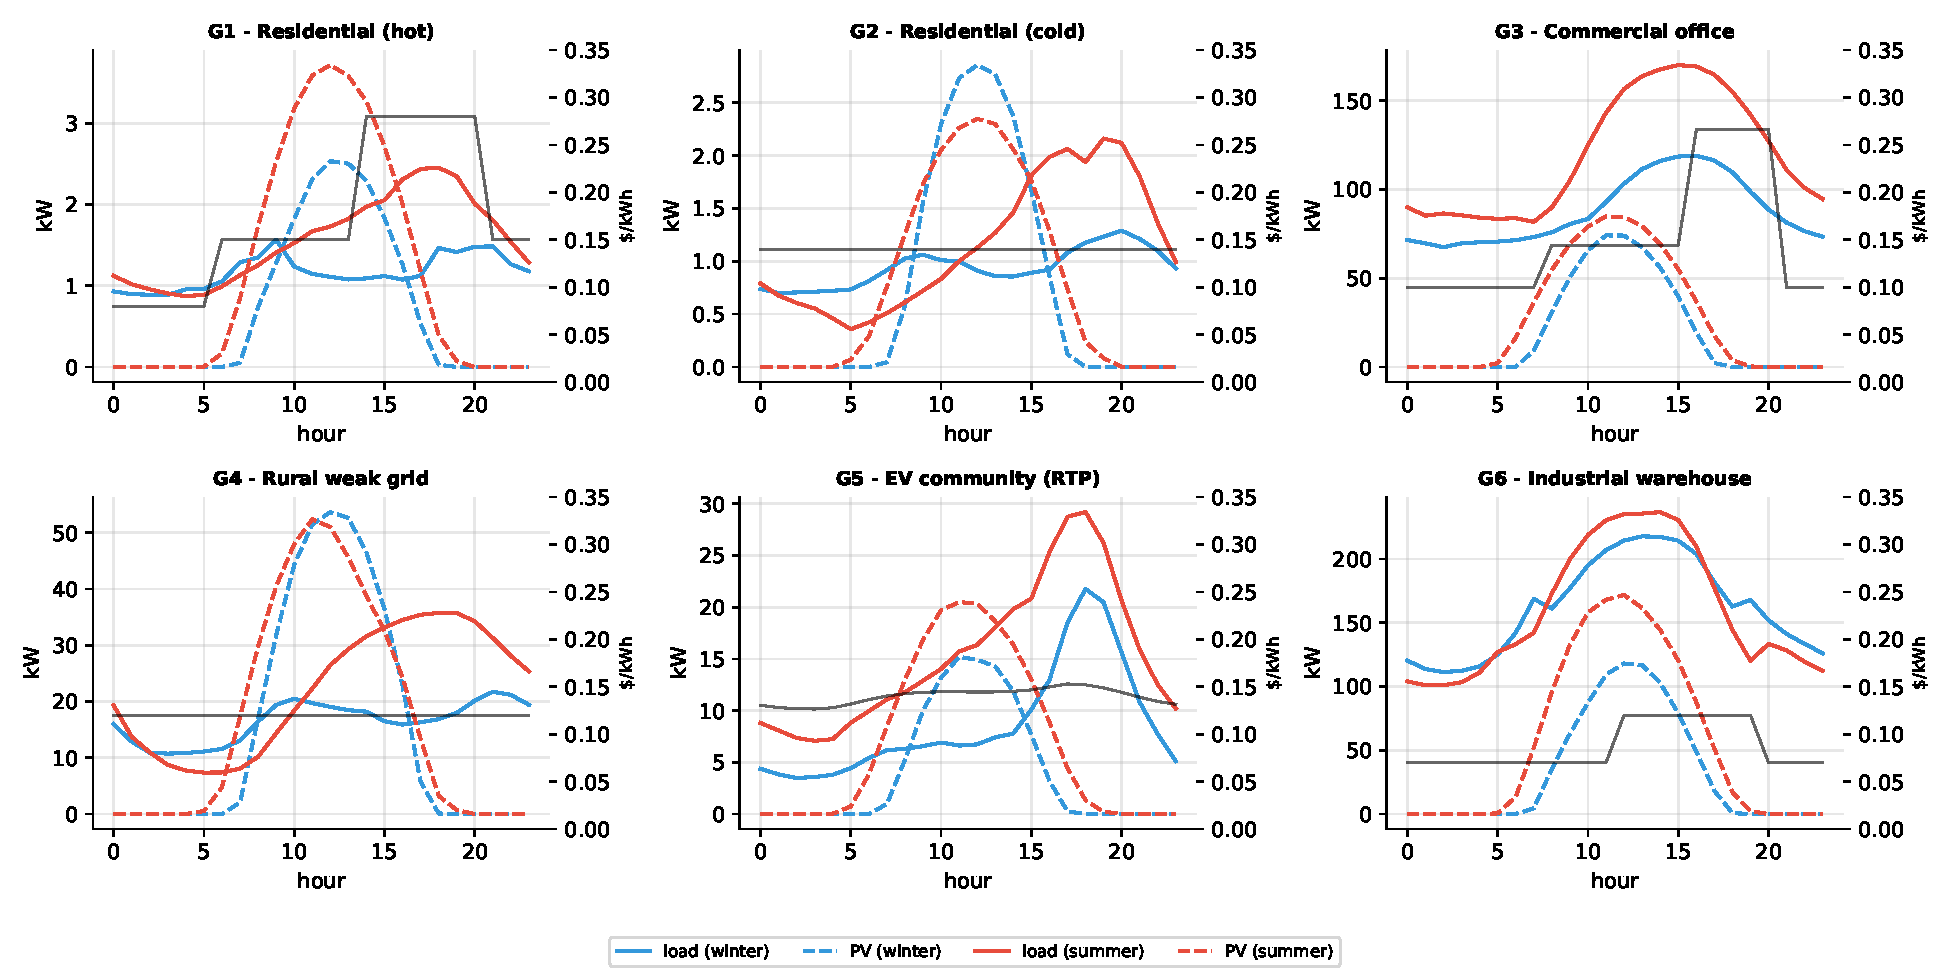
\includegraphics[width=0.92\textwidth]{figures/fig_dataset_profiles.pdf}
\caption{Mean winter (blue) and summer (red) load (solid) and PV (dashed) per
archetype, with the import price (grey, right axis).}
\label{fig:data}
\end{figure*}

% ---------------------------------------------------------------------
\section{Methods}

\subsection{Observation and action}
The 143-dimensional observation contains:
\begin{itemize}
\item the current state (7): SOC, net load, price, hour encoding, previous action and last forecast error;
\item a 4-step history of net load;
\item a 24\,h forecast window of net load, price, PV and hour encoding (120), which keeps the 131-dimensional layout of the original study;
\item a 9-feature \emph{grid descriptor}: storage hours, ramp agility, PV and load relative to inverter rating, export value, demand-charge intensity, import and export headroom, and degradation cost;
\item 3 context features: the day's peak net load, the day's peak price and the running peak import.
\end{itemize}
All features are dimensionless, so a single network can read any grid. The action is
$a_t\in[-1,1]$, scaled by $\bar P$.

\subsection{GPU-batched environment}
The environment holds the state of $N$ microgrids as PyTorch tensors. Every
grid's year of profiles sits on the GPU, each environment samples a training
day per episode, and one batch can mix grids. Episodes have a fixed 24 steps, so
all environments reset together. A unit test checks that, with the original
efficiency-agnostic SOC limits enabled, \G{G1} reproduces the original
Gymnasium environment to within $6\times10^{-5}$\,\$ per episode. By default we use the
exact SOC limits $E+\eta_c P^{ch}\le E^{\max}$ and $E-P^{dis}/\eta_d\ge E^{\min}$,
because the original limits let the battery gain up to 5\,\% of free energy near
empty. Forecast error is AR(1) noise with $\rho=0.9$ applied to the realised
load and PV, so an hour that is badly forecast tends to stay badly forecast.

\subsection{Agents}
\textit{SAC} uses twin Q-networks, automatic entropy tuning (target entropy
$-1$), $256\times256$ MLPs, a $5\times10^5$ GPU replay buffer, 128 parallel
environments, 4 gradient updates per vector step with batch 1024, and
$\gamma=1$ over the finite 24\,h horizon. The update block is captured in a CUDA
graph with fused Adam, which brings a 6M-step run to about 12 minutes.
\textit{PPO} uses a tanh-squashed Gaussian policy, GAE ($\lambda=0.95$), 512
environments, clip 0.2 and 10M steps. \textit{R-SAC} is SAC trained with a forecast
error level drawn uniformly from $[0,30]$\,\% in every episode. The
\textit{generalist} SAC trains on all six grids at once with 1.5$\times$ the
budget. The \textit{zero-shot} SAC is trained on five grids and evaluated on the
sixth. A running mean/variance normaliser is fitted to the observations.
Features that never vary during training (for example a specialist's constant
grid descriptor) are only centred, not scaled; otherwise unseen variation is
amplified about $10^4$ times (Section~\ref{sec:disc}). Every run keeps the
checkpoint with the best validation-day score, defined as the mean ratio of
cost to NoOp cost over its training grids. Test days are used only for
reporting.

\subsection{Baselines}
\begin{itemize}
\item \textbf{LP (oracle).} An LP over charge, discharge, import, export, shed load, curtailment, peak-excess and running-peak variables. Its objective equals the environment's daily cost, including the terminal penalty and ramp limits, and a test confirms that the LP objective matches the executed cost on every grid. Given the actual day, it is the true optimum.
\item \textbf{LP (open loop).} The same LP planned on the forecast and executed without revision.
\item \textbf{MPC.} A shrinking-horizon LP that re-solves every hour on the forecast of the remaining hours, starting from the measured state, and applies the first action.
\item \textbf{Heuristics.} NoOp (idle battery), the original price-threshold rule, and a self-consumption controller.
\end{itemize}

\subsection{Metric and statistics}
The headline metric is the share of the oracle LP's savings that a method
captures,
\begin{equation}
\mathrm{Capture} = 100\cdot\frac{\bar c_{\mathrm{NoOp}}-\bar c_{m}}{\bar c_{\mathrm{NoOp}}-\bar c_{\mathrm{LP}}}\ \% ,
\end{equation}
where $\bar c$ is the mean daily cost over the test days. A capture of 100 is
optimal, 0 is no better than an idle battery, and negative values are worse than
idle. The metric makes grids whose daily costs differ by three orders of
magnitude comparable. We report the mean $\pm$ standard deviation over two
training seeds and use Wilcoxon signed-rank tests~\cite{wilcoxon1945} on paired
test days. All runs start at 50\,\% SOC.

% ---------------------------------------------------------------------
\section{Results}

The full study, with 44 trained agents and all evaluations, took 7.6\,h on a single RTX~3050
laptop GPU (4\,GB).

\subsection{Phase 1: single-home baseline}
On the original single-home day (Pecan Street data, Stable-Baselines3 agents,
25 episodes), the mean daily profit was:
\begin{itemize}
\item LP: $-\$1.94$;
\item R-SAC: $-\$2.35$;
\item SAC: $-\$2.59$;
\item PPO: $-\$5.11$;
\item NoOp: $-\$11.00$.
\end{itemize}
With 30\,\% forecast error, R-SAC ($-\$3.04$) overtook the open-loop LP ($-\$3.19$).
This study had only one day of data, no MPC and no generalisation test, and those
are the limits that motivated the multi-grid extension.

\subsection{E1: per-grid specialists}
Table~\ref{tab:capture} and Fig.~\ref{fig:e1} give the results for a clean
forecast. MPC matches the oracle LP to within float tolerance at 0\,\% error, so
it serves as a second optimum. Specialist SAC captures 92\,\% (\G{G3}), 97\,\%
(\G{G4}), 81\,\% (\G{G6}), 78\,\% (\G{G1}) and 67\,\% (\G{G5}) of the optimal
savings. On the weak-grid \G{G4}, SAC reduces shed load from 4.45\,kWh/day
(NoOp) to 0.03\,kWh/day. \G{G2} is the hard case. Its flat tariff leaves only
self-consumption value, the margin over NoOp is small (\$0.33/day), and SAC
reaches 37\,\% with the largest spread between seeds. PPO is far weaker,
falling below NoOp on \G{G2} and \G{G5}, which matches the gap seen in the
single-home study. The two heuristics are poor across sites. The original rule
loses money on every grid, because it was tuned for one tariff. Self-consumption helps
the homes but is harmful under demand charges and grid caps. Every learned and
heuristic controller is significantly worse than MPC on every grid
($p<10^{-12}$, Wilcoxon signed-rank on paired test days).

\begin{table*}[t]
\centering
\caption{E1--E3: share of the perfect-foresight LP's savings captured on held-out test days
(\%, mean $\pm$ s.d.\ over 2 seeds; clean forecast). Zero-shot = trained on the
other five grids (1 seed).}
\label{tab:capture}
\begin{tabular}{lrrrrrr}
\toprule
Method & G1 & G2 & G3 & G4 & G5 & G6 \\
\midrule
LP (oracle) / MPC & 100.0 & 100.0 & 100.0 & 100.0 & 100.0 & 100.0 \\
SAC (specialist) & \textbf{77.8} $\pm$ 1.1 & \textbf{36.6} $\pm$ 6.9 & \textbf{92.2} $\pm$ 0.4 & \textbf{97.3} $\pm$ 0.2 & \textbf{66.6} $\pm$ 4.3 & \textbf{81.2} $\pm$ 0.4 \\
Generalist SAC (one policy) & 72.7 $\pm$ 0.5 & 15.2 $\pm$ 3.5 & 88.6 $\pm$ 2.1 & 94.2 $\pm$ 2.0 & 60.9 $\pm$ 3.2 & 79.4 $\pm$ 0.6 \\
PPO (specialist) & 34.7 $\pm$ 0.9 & $-$104.0 $\pm$ 14.0 & 57.0 $\pm$ 16.3 & 85.7 $\pm$ 0.1 & $-$82.9 $\pm$ 39.1 & 58.0 $\pm$ 4.1 \\
Zero-shot SAC (unseen grid) & $-$487.8 & $-$141.0 & $-$17.2 & $-$7.7 & $-$67.6 & $-$79.3 \\
Self-consumption rule & 9.6 & 27.5 & $-$37.0 & $-$82.8 & 21.6 & $-$72.5 \\
Original rule-based & $-$1849.6 & $-$4558.9 & $-$824.0 & $-$967.5 & $-$2568.5 & $-$1328.2 \\
\bottomrule
\end{tabular}
\end{table*}

\begin{figure*}[t]
\centering
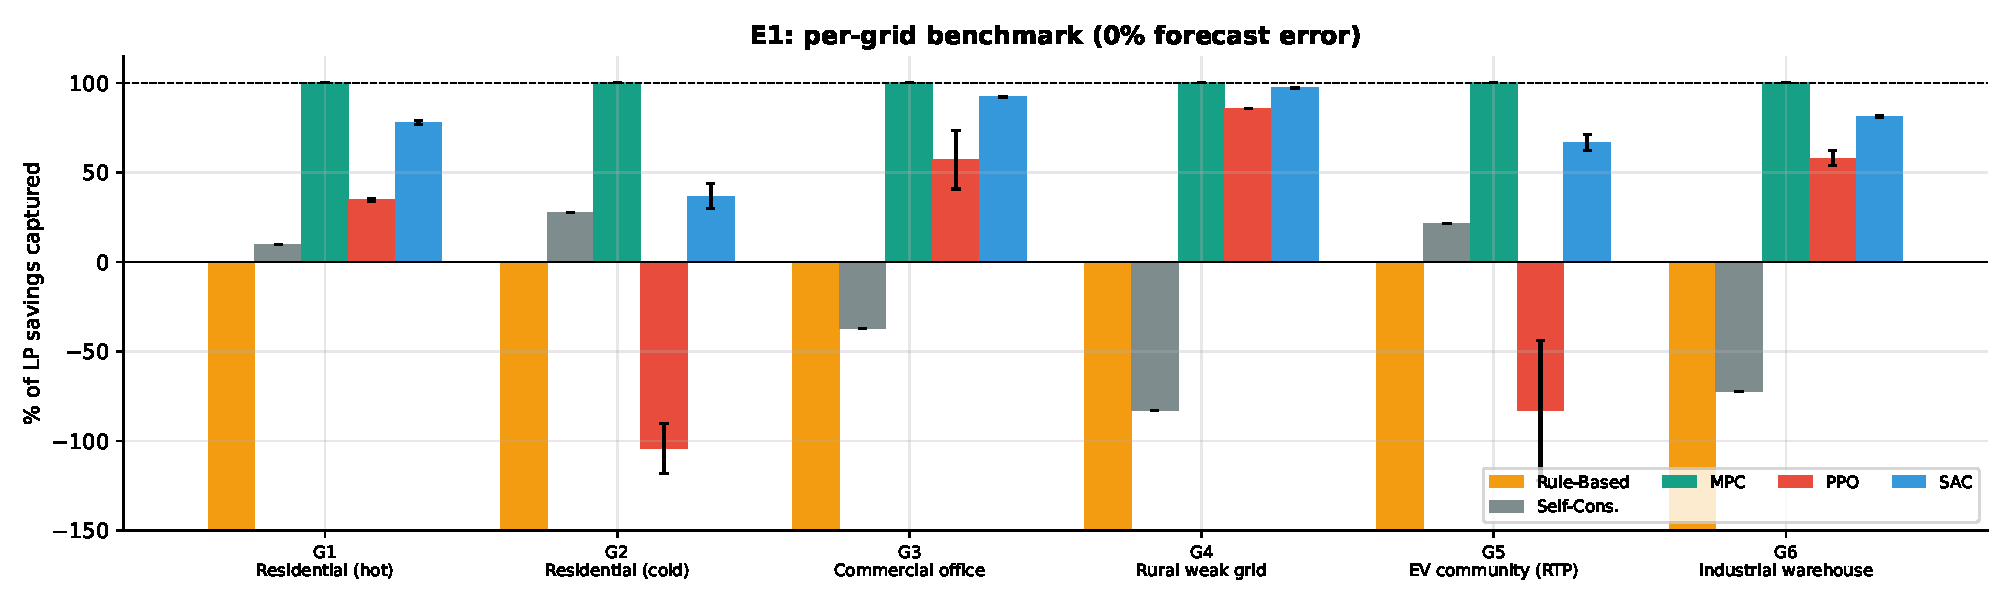
\includegraphics[width=0.95\textwidth]{figures/fig_e1_per_grid.pdf}
\caption{E1: per-grid benchmark at 0\,\% forecast error (error bars: s.d.\ over seeds;
the rule-based bars extend below the axis).}
\label{fig:e1}
\end{figure*}

\subsection{E2: one generalist policy}
A single SAC policy that reads the grid descriptor controls all six grids. It
stays within 2--6 points of the specialists on \G{G1} and \G{G3}--\G{G6}
(Fig.~\ref{fig:e2e3}). The exception is again \G{G2} (15 vs.\ 37), where the
small value at stake is easily outweighed by the larger-cost grids in the shared
training signal. One deployable network for every site type is therefore
feasible within the distribution it was trained on.

\begin{figure*}[t]
\centering
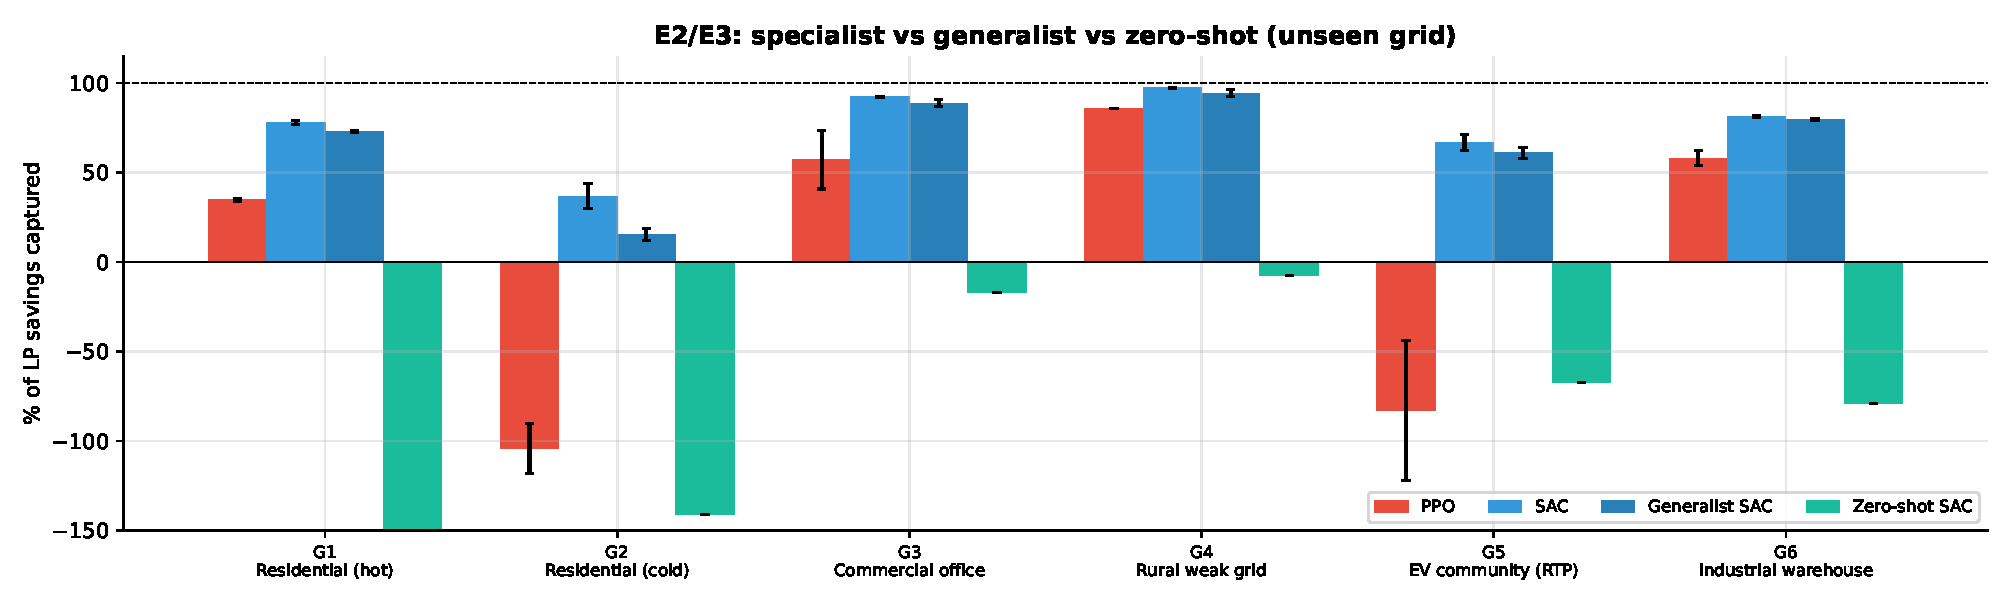
\includegraphics[width=0.95\textwidth]{figures/fig_e2_e3_generalisation.pdf}
\caption{E2/E3: specialist PPO and SAC, the generalist SAC trained on all grids, and the zero-shot
SAC trained on the other five grids.}
\label{fig:e2e3}
\end{figure*}

\begin{figure}[t]
\centering
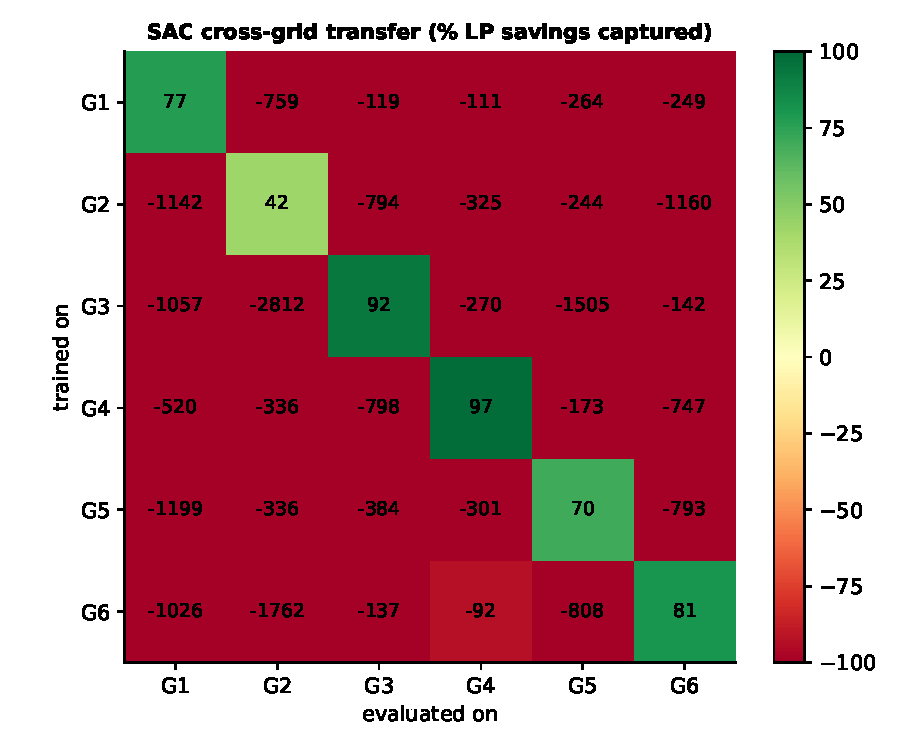
\includegraphics[width=0.85\columnwidth]{figures/fig_e3_transfer_sac.pdf}
\caption{E3: SAC specialist trained on the row grid and evaluated unchanged on the column grid
(\% of LP savings captured, seed 0; colour clipped at $\pm100$).}
\label{fig:transfer}
\end{figure}

\begin{figure*}[t]
\centering
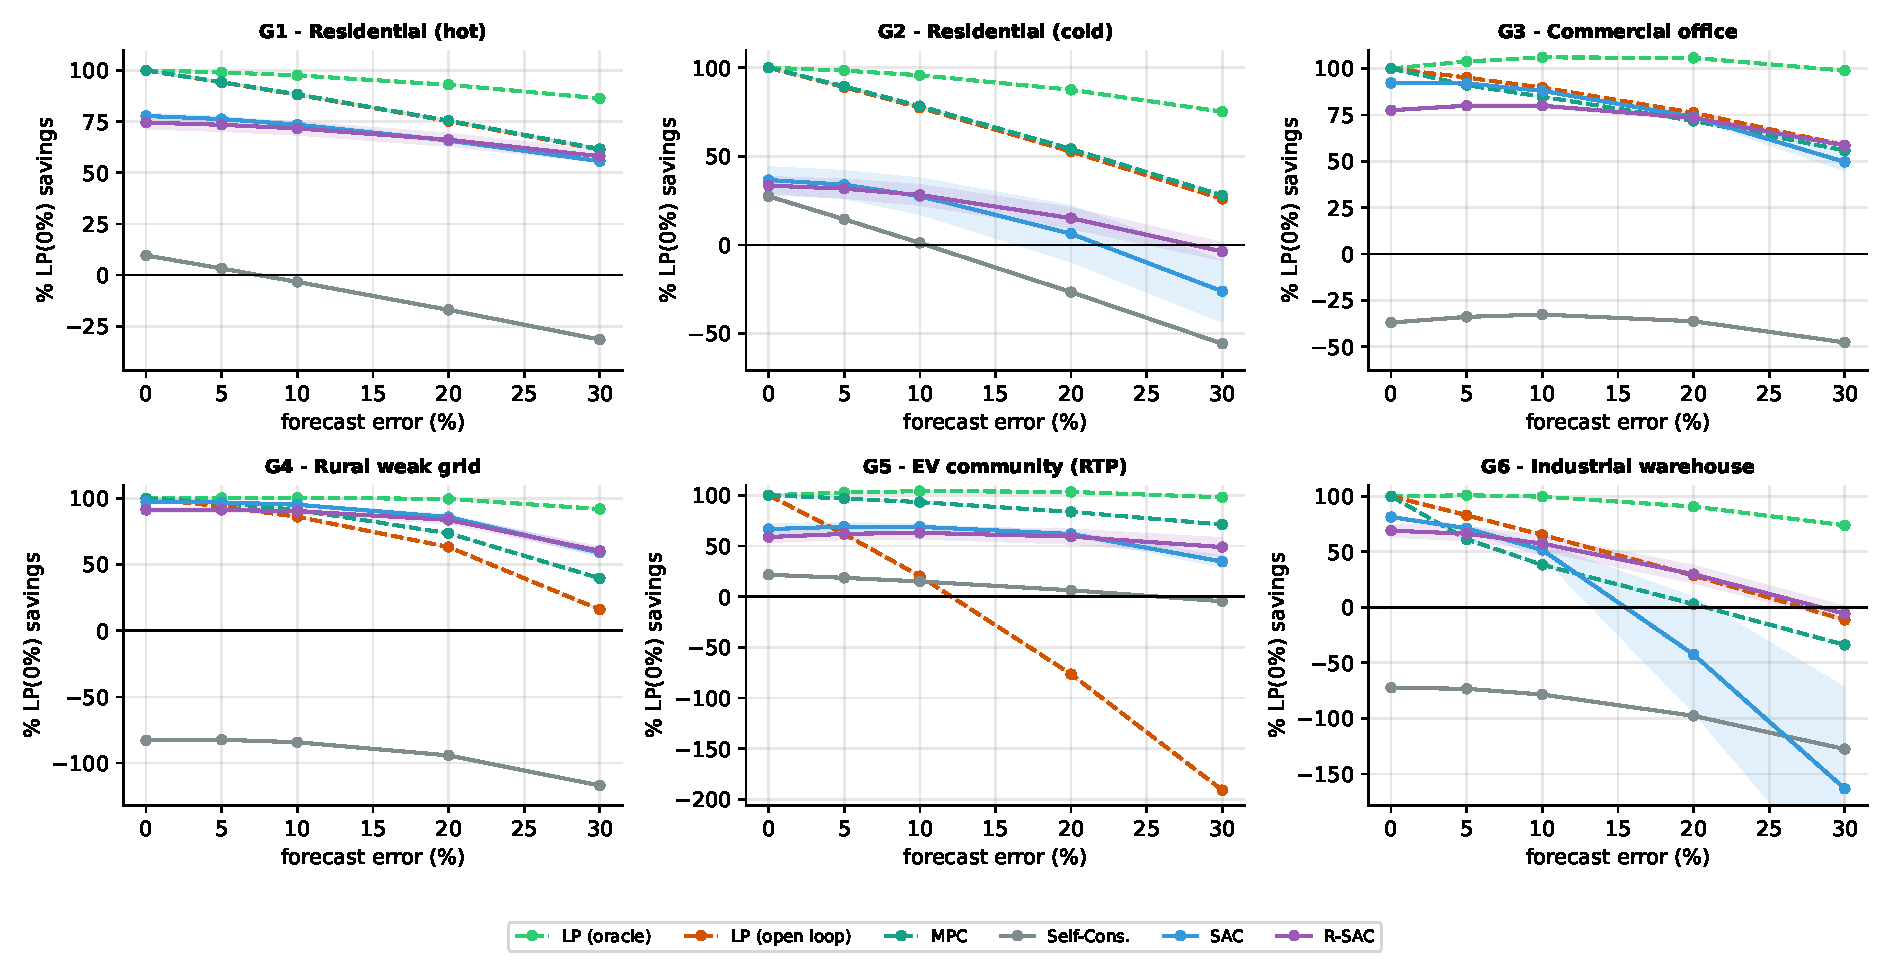
\includegraphics[width=0.95\textwidth]{figures/fig_e4_robustness.pdf}
\caption{E4: share of the clean-forecast LP's savings kept as correlated forecast error grows
(bands: s.d.\ over seeds). The LP oracle curve plans on the realised day.}
\label{fig:e4}
\end{figure*}

\begin{figure*}[t]
\centering
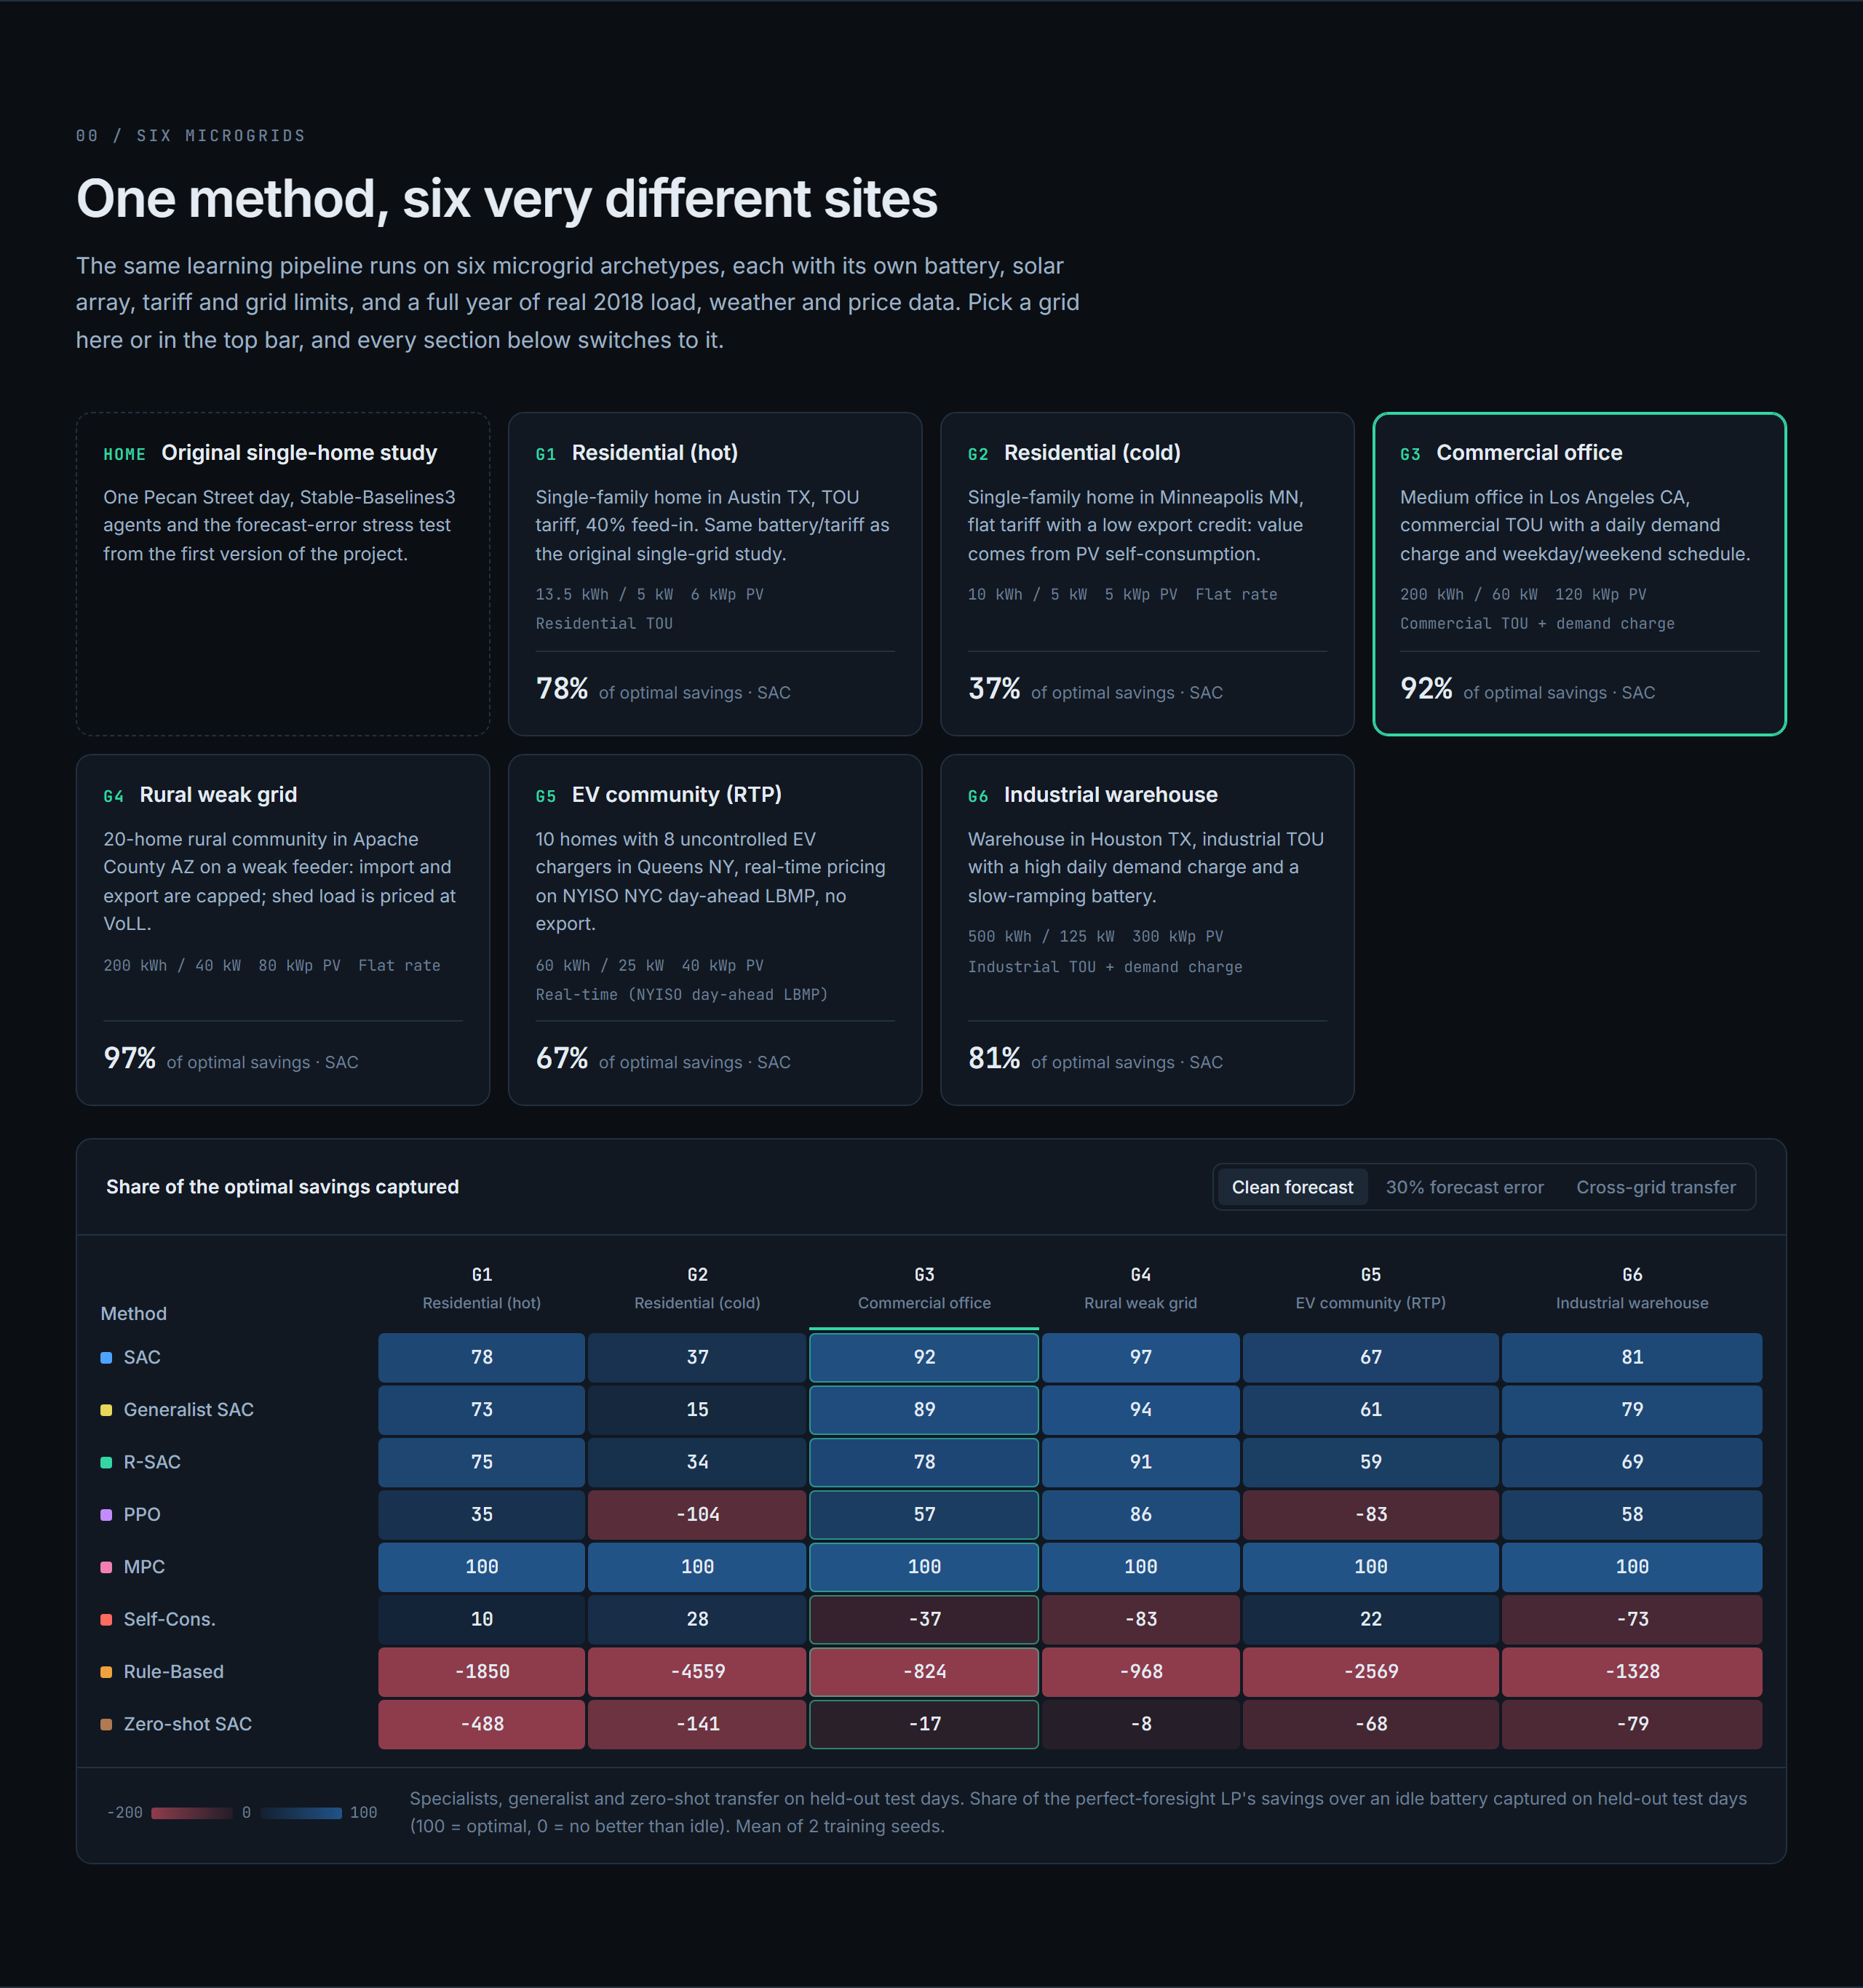
\includegraphics[width=0.49\textwidth]{figures/dashboard_grids.png}\hfill
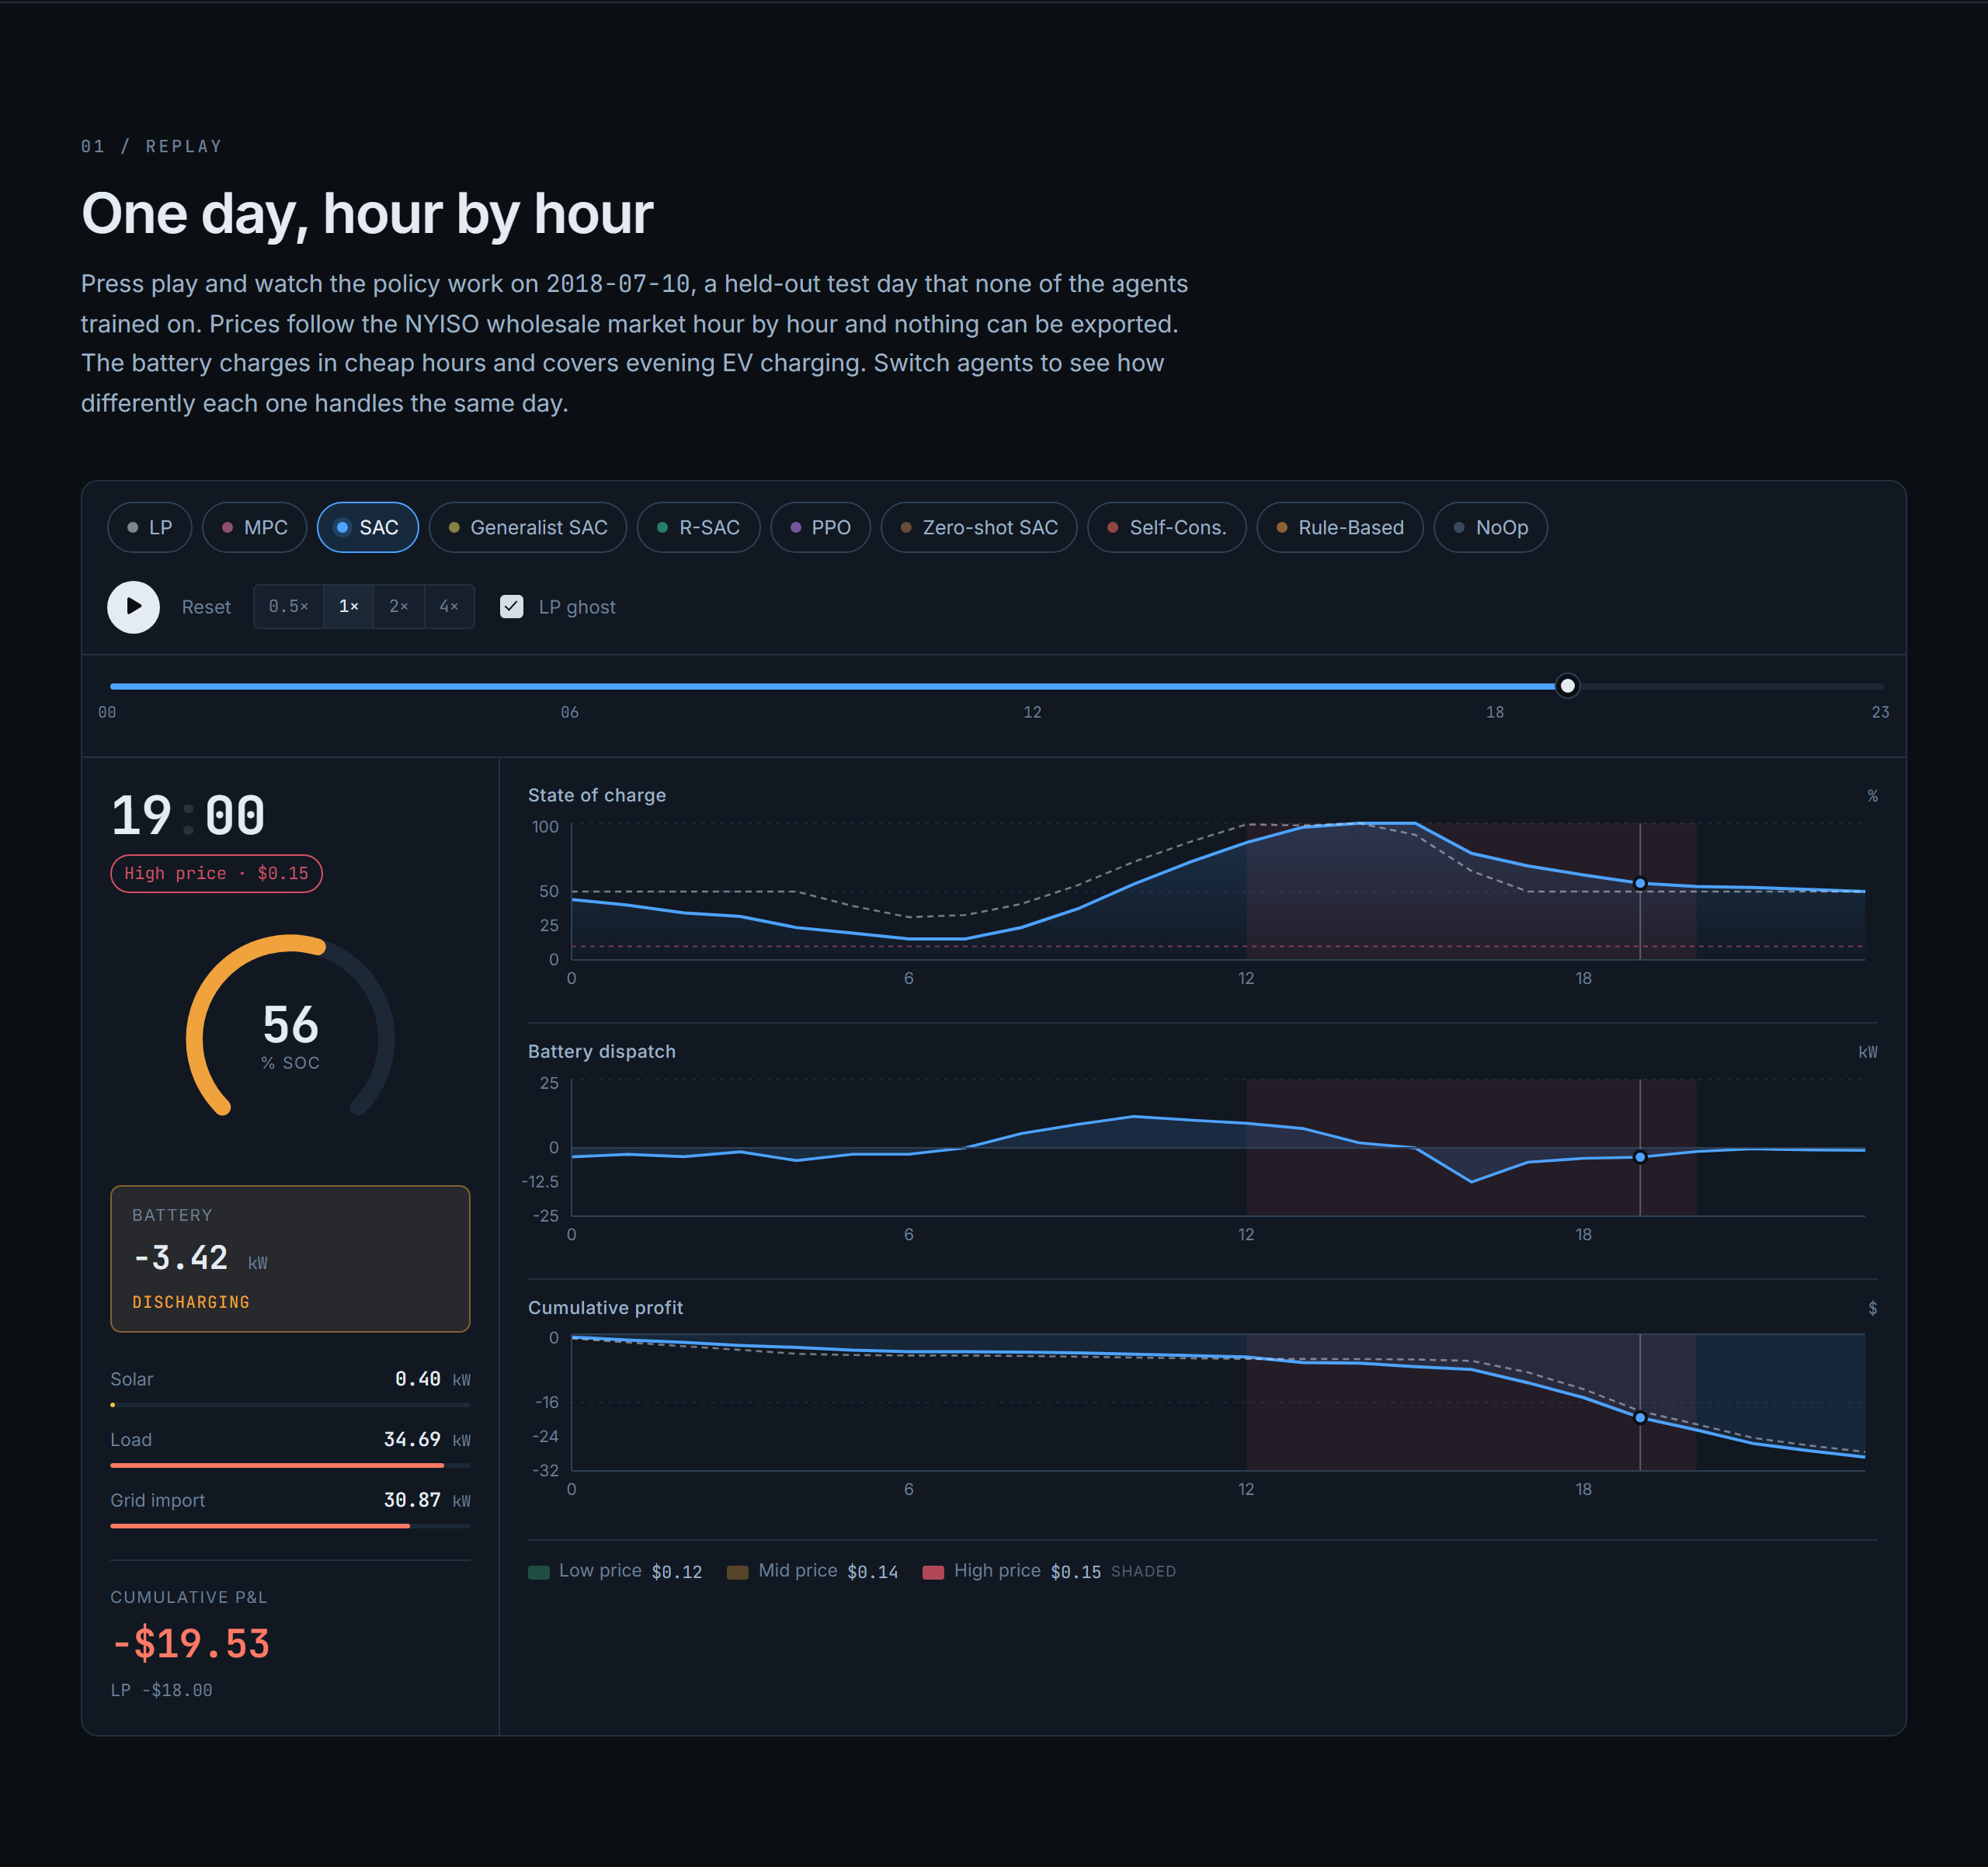
\includegraphics[width=0.49\textwidth]{figures/dashboard_replay_g5.png}
\caption{Interactive dashboard. Left: the grid selector and the cross-grid capture
table. Right: hour-by-hour replay of SAC on a \G{G5} test day (real-time prices),
with the LP plan as a dashed ghost line.}
\label{fig:dash}
\end{figure*}

\subsection{E3: transfer to an unseen grid}
Generalisation outside the training set fails. Leave-one-grid-out SAC is worse
than an idle battery on every held-out grid. It comes closest on \G{G4} ($-8$) and
\G{G3} ($-17$), and does worst on \G{G1} ($-488$), whose economics are the
smallest in absolute terms. The specialist transfer matrix
(Fig.~\ref{fig:transfer}) is strongly negative off the diagonal, so each policy
encodes its own tariff and limits. With only five training configurations, the
descriptor space is too sparse to interpolate. This is a limitation of the
present study, not evidence that RL cannot generalise. Training on many
procedurally generated configurations is the natural next step.


\subsection{E4: robustness to forecast error}
Fig.~\ref{fig:e4} and Table~\ref{tab:e4} measure every method against the
clean-forecast oracle of the same days, with three AR(1) error draws per noise level for
each of the two seeds. Three regimes appear:
\begin{itemize}
\item \textbf{Real-time prices} (\G{G5}). The open-loop LP collapses to $-191$\,\%. A
schedule fixed before the day starts cannot react when the realised PV and load
diverge from the forecast. MPC (71\,\%) is clearly best here.
\item \textbf{Homes} (\G{G1}, \G{G2}). MPC and the open-loop LP degrade
almost identically and stay ahead of SAC.
\item \textbf{Demand charges and grid caps} (\G{G3}, \G{G4}, \G{G6}). A single
wrong hour sets the daily peak or sheds load, and here the domain-randomised R-SAC is
best: 58.5 vs.\ 55.8 for MPC on \G{G3}, 60.3 vs.\ 39.6 on \G{G4}, and $-5.8$ vs.\
$-33.9$ on \G{G6}. A likely reason is that the correlated error keeps MPC's
forecast biased for several hours, so each re-plan misjudges the peak hour
again, and every misjudged hour raises the running peak.
\end{itemize}
Plain SAC degrades smoothly on most grids but fails on \G{G6} at high error
($-163$\,\%), because a policy that has only seen perfect forecasts has never
learned what a missed peak costs. Domain randomisation removes this failure.

\begin{table}[t]
\centering
\caption{E4: \% of the clean-forecast LP's savings kept at 30\,\% forecast error
(mean of 2 seeds $\times$ 3 error draws). Best per grid in bold.}
\label{tab:e4}
\setlength{\tabcolsep}{4pt}
\begin{tabular}{lrrrrrr}
\toprule
Method & G1 & G2 & G3 & G4 & G5 & G6 \\
\midrule
LP (open loop) & 61.3 & 26.0 & \textbf{58.6} & 16.0 & $-$190.8 & $-$11.4 \\
MPC & \textbf{61.6} & \textbf{27.9} & 55.8 & 39.6 & \textbf{71.1} & $-$33.9 \\
SAC & 55.7 & $-$26.2 & 49.7 & 59.0 & 34.6 & $-$163.4 \\
R-SAC & 58.1 & $-$3.7 & 58.5 & \textbf{60.3} & 48.9 & \textbf{$-$5.8} \\
\bottomrule
\end{tabular}
\end{table}

% ---------------------------------------------------------------------
\section{Discussion and Limitations}
\label{sec:disc}

\textit{Which controller should be deployed?} With good forecasts, MPC is
optimal and should be preferred. With poor forecasts, the answer depends on the
site. MPC remains best for homes and real-time prices, while
uncertainty-trained RL is best where costs are driven by one peak hour or by a
hard grid limit. This site dependence is the main finding of the study, and it
could not have been observed with one microgrid.

\textit{An evaluation pitfall.} Our first robustness evaluation showed SAC
collapsing already at 5\,\% forecast error. The cause was the observation
normaliser. The forecast-error input is exactly zero throughout noise-free
training, so its fitted variance was ${\sim}5\times10^{-10}$, and any non-zero
error at test time was amplified ${\sim}10^4$ times into the clip limit.
Normalising constant features by centring only removed the artefact without retraining.
The clean-forecast results (E1, E2) were unchanged. We report this because the same
artefact can make any RL controller appear brittle in robustness studies.

\textit{Limitations.}
\begin{itemize}
\item We use two training seeds (one for E3), so the confidence intervals are wide, especially on \G{G2}.
\item The data cover one year and US sites only.
\item EV sessions are synthetic.
\item Forecast error perturbs load and PV but not prices.
\item The horizon is one day with a soft terminal SOC target.
\item Battery ageing is linear in throughput.
\end{itemize}

% ---------------------------------------------------------------------
\section{Conclusion and Future Work}
We extended a single-home RL battery study to six heterogeneous microgrids with
real 2018 data, a GPU-batched simulator, an exact LP and an hourly MPC.
\begin{itemize}
\item SAC specialists capture 67--97\,\% of the optimal savings on five of the six grids.
\item One generalist policy serves all six grids at a small cost.
\item Zero-shot transfer to an unseen grid fails.
\item Under forecast error, MPC is preferable for homes and real-time prices, while domain-randomised SAC is preferable under demand charges and weak-grid limits.
\end{itemize}
Future work will train on procedurally generated configurations to make
zero-shot transfer possible, add price-forecast uncertainty and multi-day horizons,
and study hybrid controllers that use RL to correct MPC.

% ---------------------------------------------------------------------
\section*{Implementation, Code and Data Availability}
All code, trained-model results, figures and the dashboard are available at
\url{https://github.com/Shreyansh-023/AIFS-MicroGrid-Project}.
\begin{itemize}
\item \textbf{Environment.} Python~3.10, PyTorch~2.6 (CUDA~12.4), NumPy, SciPy~1.15 (HiGHS), pandas and pyarrow. The original pipeline uses Gymnasium~0.29 and Stable-Baselines3~2.1. The dashboard uses React~19, Vite and Recharts.
\item \textbf{Hardware.} Windows~11 laptop with an NVIDIA RTX~3050 (4\,GB).
\item \textbf{Data.} All datasets download automatically without API keys. Sources are the NREL End-Use Load Profiles and weather files (OEDI S3 bucket) and NYISO public price archives.
\item \textbf{Reproduction.} The script \texttt{run\_multigrid.py} runs the full study, and \texttt{export\_multigrid\_web.py} rebuilds the dashboard data. The dashboard has a grid selector that switches every view between the six archetypes and the original single-home study (Fig.~\ref{fig:dash}).
\end{itemize}

\section*{Acknowledgment}
We thank our project supervisor for guidance and the suggestion to extend the study
to multiple microgrid configurations.

% ---------------------------------------------------------------------
\begin{thebibliography}{00}

\bibitem{vazquez2019review}
J.~R. V\'azquez-Canteli and Z.~Nagy, ``Reinforcement learning for demand
response: A review of algorithms and modeling techniques,'' \emph{Applied
Energy}, vol.~235, pp.~1072--1089, 2019.

\bibitem{parisio2014mpc}
A.~Parisio, E.~Rikos, and L.~Glielmo, ``A model predictive control approach to
microgrid operation optimization,'' \emph{IEEE Trans. Control Syst. Technol.},
vol.~22, no.~5, pp.~1813--1827, 2014.

\bibitem{haarnoja2018sac}
T.~Haarnoja, A.~Zhou, P.~Abbeel, and S.~Levine, ``Soft actor-critic:
Off-policy maximum entropy deep reinforcement learning with a stochastic
actor,'' in \emph{Proc. ICML}, 2018, pp.~1861--1870.

\bibitem{schulman2017ppo}
J.~Schulman, F.~Wolski, P.~Dhariwal, A.~Radford, and O.~Klimov, ``Proximal
policy optimization algorithms,'' arXiv:1707.06347, 2017.

\bibitem{raffin2021sb3}
A.~Raffin, A.~Hill, A.~Gleave, A.~Kanervisto, M.~Ernestus, and N.~Dormann,
``Stable-Baselines3: Reliable reinforcement learning implementations,''
\emph{J. Mach. Learn. Res.}, vol.~22, no.~268, pp.~1--8, 2021.

\bibitem{wilson2022eulp}
E.~Wilson \emph{et al.}, ``End-use load profiles for the U.S. building stock:
Methodology and results of model calibration, validation, and uncertainty
quantification,'' National Renewable Energy Laboratory, Golden, CO, Tech. Rep.
NREL/TP-5500-80889, 2022.

\bibitem{huangfu2018highs}
Q.~Huangfu and J.~A.~J. Hall, ``Parallelizing the dual revised simplex
method,'' \emph{Math. Program. Comput.}, vol.~10, no.~1, pp.~119--142, 2018.

\bibitem{vazquez2019citylearn}
J.~R. V\'azquez-Canteli, J.~K\"ampf, G.~Henze, and Z.~Nagy, ``CityLearn v1.0: An
OpenAI Gym environment for demand response with deep reinforcement learning,''
in \emph{Proc. ACM BuildSys}, 2019, pp.~356--357.

\bibitem{schulman2016gae}
J.~Schulman, P.~Moritz, S.~Levine, M.~Jordan, and P.~Abbeel, ``High-dimensional
continuous control using generalized advantage estimation,'' in \emph{Proc.
ICLR}, 2016.

\bibitem{cobbe2019quantifying}
K.~Cobbe, O.~Klimov, C.~Hesse, T.~Kim, and J.~Schulman, ``Quantifying
generalization in reinforcement learning,'' in \emph{Proc. ICML}, 2019,
pp.~1282--1289.

\bibitem{henderson2018matters}
P.~Henderson, R.~Islam, P.~Bachman, J.~Pineau, D.~Precup, and D.~Meger, ``Deep
reinforcement learning that matters,'' in \emph{Proc. AAAI}, 2018.

\bibitem{tobin2017domain}
J.~Tobin, R.~Fong, A.~Ray, J.~Schneider, W.~Zaremba, and P.~Abbeel, ``Domain
randomization for transferring deep neural networks from simulation to the
real world,'' in \emph{Proc. IEEE/RSJ IROS}, 2017, pp.~23--30.

\bibitem{makoviychuk2021isaac}
V.~Makoviychuk \emph{et al.}, ``Isaac Gym: High performance GPU-based physics
simulation for robot learning,'' in \emph{Proc. NeurIPS Datasets and
Benchmarks Track}, 2021.

\bibitem{dobos2014pvwatts}
A.~P. Dobos, ``PVWatts version 5 manual,'' National Renewable Energy
Laboratory, Golden, CO, Tech. Rep. NREL/TP-6A20-62641, 2014.

\bibitem{nyiso}
New York Independent System Operator, ``Day-ahead market LBMP -- zonal,''
[Online]. Available: \url{https://mis.nyiso.com/public/}

\bibitem{wilcoxon1945}
F.~Wilcoxon, ``Individual comparisons by ranking methods,'' \emph{Biometrics
Bulletin}, vol.~1, no.~6, pp.~80--83, 1945.

\end{thebibliography}

\end{document}
